\documentclass[11pt,twoside]{ce}

\usepackage{graphicx}
\usepackage{wrapfig}
\usepackage{color}
\usepackage{acronym}
\usepackage{hyperref}
\usepackage{newclude}
\usepackage{enumitem}
\usepackage{caption}
\usepackage{subcaption}

%Eigen toevoeging
\usepackage{listings} % Required for insertion of code
\usepackage{xcolor}
\usepackage{textcomp}

\lstset{
    inputencoding=utf8,
%    backgroundcolor=\color{white},
    tabsize=4,
    rulecolor=,
    upquote=true,
%    aboveskip={1.5\baselineskip},
    columns=fixed,
    showstringspaces=false,
    extendedchars=true,
    breaklines=true,
    prebreak = \raisebox{0ex}[0ex][0ex]{\ensuremath{\hookleftarrow}},
    frame=single,
    showtabs=false,
    showspaces=false,
    showstringspaces=false,
    basicstyle=\scriptsize\ttfamily,
    identifierstyle=\ttfamily,
    keywordstyle=\ttfamily\color[rgb]{0,0,1},
    commentstyle=\ttfamily\color[rgb]{0.133,0.545,0.133},
    stringstyle=\ttfamily\color[rgb]{0.627,0.126,0.941},
}

\makeatletter
\lstdefinelanguage{llvm}{
  morecomment = [l]{;},
  morestring=[b]", 
  sensitive = true,
  classoffset=0,
  morekeywords={
    define, declare, global, constant,
    internal, external, private,
    linkonce, linkonce_odr, weak, weak_odr, appending,
    common, extern_weak,
    thread_local, dllimport, dllexport,
    hidden, protected, default,
    except, deplibs,
    volatile, fastcc, coldcc, cc, ccc,
    x86_stdcallcc, x86_fastcallcc,
    ptx_kernel, ptx_device,
    signext, zeroext, inreg, sret, nounwind, noreturn,
    nocapture, byval, nest, readnone, readonly, noalias, uwtable,
    inlinehint, noinline, alwaysinline, optsize, ssp, sspreq,
    noredzone, noimplicitfloat, naked, alignstack,
    module, asm, align, tail, to,
    addrspace, section, alias, sideeffect, c, gc,
    target, datalayout, triple,
    blockaddress
  },
  classoffset=1, keywordstyle=\color{purple},
  morekeywords={
    fadd, sub, fsub, mul, fmul,
    sdiv, udiv, fdiv, srem, urem, frem,
    and, or, xor,
    icmp, fcmp,
    eq, ne, ugt, uge, ult, ule, sgt, sge, slt, sle,
    oeq, ogt, oge, olt, ole, one, ord, ueq, ugt, uge,
    ult, ule, une, uno,
    nuw, nsw, exact, inbounds,
    phi, call, select, shl, lshr, ashr, va_arg,
    trunc, zext, sext,
    fptrunc, fpext, fptoui, fptosi, uitofp, sitofp,
    ptrtoint, inttoptr, bitcast,
    ret, br, indirectbr, switch, invoke, unwind, unreachable,
    malloc, alloca, free, load, store, getelementptr,
    extractelement, insertelement, shufflevector,
    extractvalue, insertvalue,
  },
  alsoletter={\%},
  keywordsprefix={\%},
}
\makeatother


%-----------------------------------------------------------------------%
%           Please enter your personal details !!!                      %
%-----------------------------------------------------------------------%

\newcommand{\TITLE}{LLVM-based $\rho$-VEX compiler}
\newcommand{\AUTHOR}{Maurice Daverveldt}
\newcommand{\country}{Netherlands}
\newcommand{\city}{Utrecht}
\newcommand{\NR}{CE-MS-2014} 
\newcommand{\KEY}{}   % key words for your thesis
\newcommand{\SUBTITLE}{asd}

%-----------------------------------------------------------------------%
%            Fixed Title page - Don't change any thing here             %
%-----------------------------------------------------------------------%
\newcommand{\DATE}{\today} 
\newcommand{\LTYPE}{latex2e}
\newcommand{\reffig}[1]{Figure~\ref{#1}}
\newcommand{\reftab}[1]{Table~\ref{#1}}
\newcommand{\refsec}[1]{Section~\ref{#1}}

%-----------------------------------------------------------------------%
%  Enter the names of members in the committee,i.e. chair-person,       %
%  advisors and other members. At this moment,                          %
%  maximally 7 members signatures are supported. Be careful             %
%  with the length of the abstract (should be about 15 lines ).         %
%                                                                       %
%  Use the following format to fill in the committee memebers           %
%        " name, group, organization"
%
%        for example, Stephan Wong, CE, TU Delft                        %
%-----------------------------------------------------------------------%
\firstadvisor{dr.ir. Stephan Wong, CE, TU Delft}
\chairperson{dr.ir. K.L.M. Bertels, CE, TU Delft}
\firstmember{dr.ir. A. van Genderen, CE, TU Delft}
\secondmember{dr.ir. Guido Wachsmuth, CE, TU Delft}


%-----------------------------------------------------------------------%
%            Fixed   - Don't change any thing here                      %
%-----------------------------------------------------------------------%

\begin{document}
\pagenumbering{roman}
\pagestyle{plain}

%-----------------------------------------------------------------------%
%            Fixed cover page  - Don't change any thing here            %
%-----------------------------------------------------------------------%
\thispagestyle{empty}
%%%%%%%%%%%%%%%%%%%%%%%%%%%%%%%%%%%%%%%%%%%%%%%%%%%%%%%%%%%%%%%%%
%                                                               %
%   Standard Cover page,                                        %
%   Author: Yunfei Wu                                           %
%   Date:   07-07-2003                                          %
%   Modif.: Ronald Bos: allow for long title                    %
%   Date:   05-04-2004                                          %
%%%%%%%%%%%%%%%%%%%%%%%%%%%%%%%%%%%%%%%%%%%%%%%%%%%%%%%%%%%%%%%%%

%-----------------------------------------------------------------------%
%            Fixed part - Don't change any thing here                   %
%-----------------------------------------------------------------------%
\addtolength{\topmargin}{0.95in}

\vspace*{-6.5cm}  \hspace*{-2.2cm}
\parbox[h]{17.8cm}{

\parbox[t]{4.3cm}{\hspace{-0.8cm}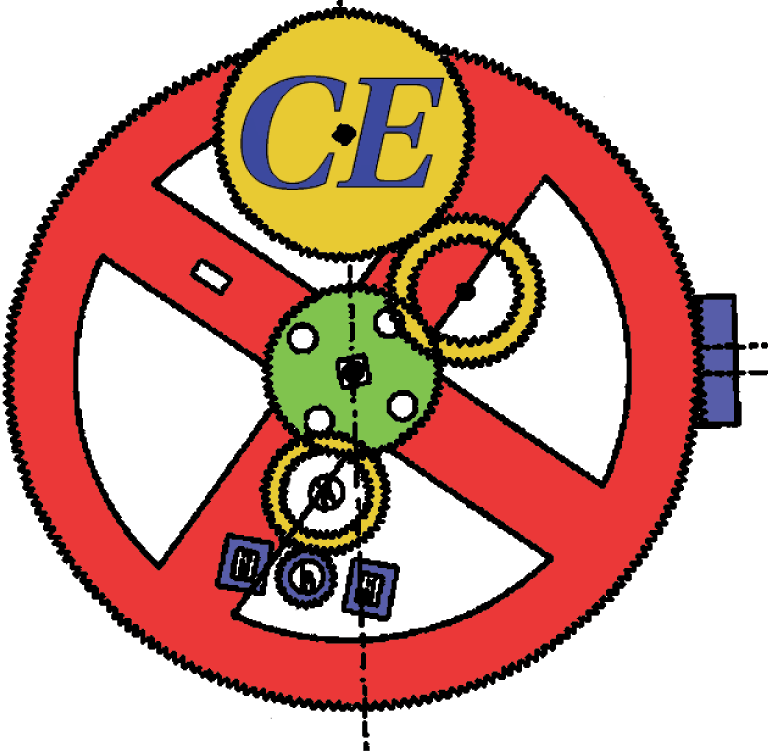
\includegraphics[width=4.5cm]{0_template/fig/CE_conv.png}}
\hspace{-0.5cm}
\parbox[b]{6cm}{\centering{\large \bf \LAB}
\\ \LABADD \\ {\bf \WEB}
\\\vspace{1.9cm}}\hfill
\parbox[b]{1.5cm}{\raggedleft{\textcolor{red}{\bf \large
\the\year}}\\\vspace{3.9cm}}
}

% begin mod Ronald Bos: removed shortstack to allow for a long title
% (longer than one line)
\hspace*{-2.8cm}
\vspace*{-0.2cm}
\parbox[h]{17.9cm}{
	\begin{center}
	\Huge{\bf MSc THESIS} \\
	\vspace*{-0.5cm}
	\textcolor{blue}{\vrule width 17.9cm height 3pt} \\
	\huge{\bf \TITLE}
	\end{center}
}
% end mod Ronald Bos

% begin mod Guido de Goede and Jonathan Hofman: Added author name, as required on cover
	\begin{center}
	\large{\bf \AUTHOR}
	\end{center}
% end mod

\vspace{0.5cm}
\hspace{8cm}{\bf \large Abstract}\\ \vspace{0.5cm}

\vspace*{15cm} \hspace*{-2.8cm}
\parbox[h]{17.8cm}{
\parbox[b]{4cm}{\hspace{-0.55cm} \includegraphics[width=4cm]{0_template/fig/TUDelft_conv.png}}
\hfill
\parbox[b]{14.2cm}{\raggedleft{\large \FAC}\\ \vspace{0.1cm}}}

\vspace*{-17.5cm}
\hspace*{-3cm}
\parbox[h]{17.9cm}{
\begin{wrapfigure}[20]{l}{6cm}
    \hspace{-0.5cm}


%----------------------------------------------------------------------------%
%   fill in  research theme logo (eps file)                                  %
%--------------------------------------------------------------------------- %
    %\centering \includegraphics[width=5cm]{logo/molen.eps}    % fill in your research theme logo %


%-----------------------------------------------------------------------%
%            Fixed part - Don't change any thing here                   %
%-----------------------------------------------------------------------%    
     \vspace{1.5cm}                %to make v-space between two figures
%     \hspace{-3.5cm}
      \unitlength 1cm
      \begin{center}
      \begin{picture}(5,1.0)      %to draw second figure by picture env.
           \put(0.0, 0.0){\framebox(4.5, 1){\bf \NR}}
           \end{picture}
          \end{center}
\end{wrapfigure}
\vspace{0.5cm}

%----------------------------------------------------------------------------%
%   fill in  the content of the abstract here (text part)                    %
%--------------------------------------------------------------------------- %
\noindent
This thesis describes the development of a LLVM-based compiler for the $\rho$-VEX processor. The $\rho$-VEX processor is a runtime reconfigurable VLIW processor. Currently, two compilers exist that target the $\rho$-VEX processor: a HP-VEX compiler and a GCC-based compiler.

We show that both compilers have disadvantages that are very difficult to fix. Therefore we have built a LLVM-based compiler that targets the $\rho$-VEX processor. The LLVM-based compiler can be parameterized in a way similar to the HP-VEX compiler. Furthermore, we will present certain optimizations that are new for LLVM-based compilers. These optimizations include a custom machine scheduler that avoids structural and data hazards in the generated binaries.

Finally, we demonstrate the operations of the LLVM-based compiler and compare the performance of generated binaries with the existing compilers. We will show that the LLVM-based compiler exceeds the performance and code quality of the GCC-based compiler. Binaries generated with the HP-VEX compiler outperform those of the LLVM-based compiler.

% FIXME put some numbers here

%-----------------------------------------------------------------------%
%            Fixed part - Don't change any thing here                   %
%-----------------------------------------------------------------------%   
}
                                   % thesis cover
\setcounter{page}{0} \cleardoublepage

%-----------------------------------------------------------------------%
%            Fixed Title page - Don't change any thing here             %
%-----------------------------------------------------------------------%
\thispagestyle{empty}
\title{\TITLE}
\subtitle{\SUBTITLE} \extitle{\EXTITLE}
\author{\AUTHOR}
\date{
    \small \LAB \\
    \small \DEP \\
    \small \FAC \\
    \small \INSTITUTE \\
} \maketitle

\setcounter{page}{0} \cleardoublepage

%-----------------------------------------------------------------------%
%       Front page includes a small abstract and signatures of          %
%       advisor, supervisor and mentors                                 %
%                                                                       % 
%       Please fill in your dedication words                            %
%-----------------------------------------------------------------------%
%%%%%%%%%%%%%%%%%%%%%%%%%%%%%%%%%%%%%%%%%%%%%%%%%%%%%%%%%%%%%%%%%
%                                                               %
%   Standard title page, no modifications required              %
%   Author: Wiebe Cnossen                                       %
%   Date:   August 11 1994                                      %
%%%%%%%%%%%%%%%%%%%%%%%%%%%%%%%%%%%%%%%%%%%%%%%%%%%%%%%%%%%%%%%%%
%   Modified by Bao Linh Dang                                   %
%   Date: 15/4/2003                                             %
%   Modified by Ronald Bos: allow long TITLE                    %
%   Date: 5/4/2004                                              %
%   Put your abstract here(about 15 lines) and the rest should  %
%   not be changed !!!                                          %
%%%%%%%%%%%%%%%%%%%%%%%%%%%%%%%%%%%%%%%%%%%%%%%%%%%%%%%%%%%%%%%%%

%-----------------------------------------------------------------------%
%            Fixed part - Don't change any thing here                   %
%-----------------------------------------------------------------------%
\thispagestyle{plain} \cleardoublepage

\topmargin -0.5in

% Ronald Bos: removed shortstack and some font size tweaking
% to allow a long TITLE (longer than one line)
\begin{center}
\huge \TITLE{} \\
\normalsize
\rule{5.5in}{1.5pt}
\vskip 0.5cm
by~\AUTHOR

\vskip 0.5cm {\bf Abstract}
\end{center}

% Start your abstract here 

\begin{small}
%------------------------------------------------------------------------%
%   Please fill in 
%       1) the first letter of the first word of your thesis abstract    %
%          into the first brace after \drop command                      %
%       2) the left letters of the first word of your thesis abstract    %
%          into the second brace                                         %
%       3) the left part of your thesis abstract after the second brace  %
%                                                                        %
%------------------------------------------------------------------------%
\
This thesis describes the development of a LLVM-based compiler for the $\rho$-VEX processor. The $\rho$-VEX processor is a runtime reconfigurable VLIW processor. Currently, two compilers exist that target the $\rho$-VEX processor: a HP-VEX compiler and a GCC-based compiler.

We show that both compilers have disadvantages that are very difficult to fix. Therefore we have built a LLVM-based compiler that targets the $\rho$-VEX processor. The LLVM-based compiler can be parameterized in a way similar to the HP-VEX compiler. Furthermore, we will present certain optimizations that are new for LLVM-based compilers. These optimizations include a custom machine scheduler that avoids structural and data hazards in the generated binaries.

Finally, we demonstrate the operations of the LLVM-based compiler and compare the performance of generated binaries with the existing compilers. We will show that the LLVM-based compiler exceeds the performance and code quality of the GCC-based compiler. Binaries generated with the HP-VEX compiler outperform those of the LLVM-based compiler.

% FIXME put some numbers here

\end{small}                                       % End of your abstract. 

% End of your abstract. The next part is fixed, don't change anything
%-----------------------------------------------------------------------%
%            Fixed part - Don't change any thing here                   %
%-----------------------------------------------------------------------%
\vskip 15pt
\begin{flushleft}
\begin{sloppypar}
\begin{tabular}{lll}
{\bf Laboratory }&:& \begin{minipage}[t]{9cm}
   {Computer Engineering}\end{minipage}    \\
{\bf Codenumber }&:& \NR         \\ \\
{\bf Committee Members }&:&
\end{tabular}
\end{sloppypar}
\end{flushleft}

\signaturepage \addtolength{\topmargin}{0.5in}
%\end{document}

\cleardoublepage

\dedicate{Dedicated to my family and friends}                                        % fill in your dedication words  

\thankyou                                          % "Thankyou" page
\tableofcontents                                   %  Table of contents

%------------------------------------------------------------------------%
%        List of Figures and Tables - don't change anything here         %
%------------------------------------------------------------------------%
%\clearsinglepage
\clearpage
\listoffigures
\addcontentsline{toc}{chapter}{List of Figures}

%\clearsinglepage
\clearpage
\listoftables
\addcontentsline{toc}{chapter}{List of Tables}

\clearpage
\chapter*{List of Acronyms}
\begin{acronym}
\acro{ALU}{Arithmetic Logic Unit}
\acro{AST}{Abstract Syntax Tree}
\acro{CPI}{Clocks Per Instruction}
\acro{DAG}{Directed Acyclic Graph}
\acro{DFA}{Deterministic Finite Automaton}
\acro{DSL}{Domain-specific Language}
\acro{FP}{Floating-point}
\acro{FU}{Functional Unit}
\acro{GCC}{GNU Compiler Collection}
\acro{IDE}{Integrated Development Environment}
\acro{ILP}{Instruction Level Parallelism}
\acro{IPC}{Instructions Per Clock}
\acro{IR}{Intermediate Representation}
\acro{ISA}{Instruction Set Architecture}
\acro{ISD}{Instruction SelectionDAG}
\acro{JIT}{Just-in-time compilation}
\acro{LLVM}{Low Level Virtual Machine}
\acro{MBB}{Machine Basic Block}
\acro{MI}{Machine Instruction}
\acro{OoO}{Out-of-Order Execution}
\acro{PC}{Program Counter}
\acro{RAW}{Read After Write}
\acro{RISC}{Reduced Instruction Set Computer}
\acro{SSA}{Single Static Assignment}
\acro{VEX}{VLIW Example}
\acro{VLIW}{Very Long Instruction Word}
\end{acronym}
\addcontentsline{toc}{chapter}{List of Acronyms}

%-----------------------------------------------------------------------%
%                     Include thesis acknowledgements                   %
%-----------------------------------------------------------------------%
% Thesis Acknowledgements ----------------------------------------------
%-----------------------------------------------------------------------%
%            Fixed part - Don't change any thing here                   %
%-----------------------------------------------------------------------%

%\begin{flushleft}
%\begin{Huge}{Acknowledgements}
%\end{Huge}
%\end{flushleft} \vskip 2cm

\nonumchapter{Acknowledgements}                        %{ACKNOWLEDGEMENTS}
\vskip 1cm
%-----------------------------------------------------------------------%
%     Please fill in your acknowledgements here                         %
%-----------------------------------------------------------------------%
In 2007 I have started studying Electronic Engineering and Design at the University of applied sciences Utrecht. After graduating in 2011 I decided to persue a degree in Computer Engineering at the Technical University Delft. This thesis reflects the new things I have learned since beginning my study at the Electrical Engineering Department.

First I would like to thank my advisor Stephan Wong for giving me the opportunity and advising me during the writing of this thesis.

Secondly I would like to thank Roël Seedorf, Anthony Brandon and Joost Hoozemans for their discussions and help during the realization of this project. Their advice has proven to be priceless.

I would like to thank my friends and family for all the support they have given me over the years.
%-----------------------------------------------------------------------%
%      no change here                                                    %
%-----------------------------------------------------------------------%

\vskip 2cm
\noindent \AUTHOR \\
\PLACE \\
\DATE

                                     % inlcude acknowledgements page

\addtocontents{toc}{\protect\addvspace{1cm}}
\cleardoublepage

\pagestyle{headings}
\pagestyle{private}
\pagenumbering{arabic}

%-----------------------------------------------------------------------%
%                     Include separate chapters                         %
%                                                                       %
%       1)  fill in the tex file of each chapter                        %
%       2)  If more chapters, add more include commands                 %
%-----------------------------------------------------------------------%

\chapter{Introduction}
\label{chap:introduction}
<INTRODUCTIE TEKST>
\section{Motivation}
% \subsection{Origin and history}
In 2008 Thijs van As designed the first version of the $\rho$-VEX processor \cite{As:2008rt}. This processor uses a VLIW design and is based on the VEX ISA. The VEX ISA is a derivative of the Lx family of embedded VLIW processors \cite{854391} from HP/STMicroelectronics.
Around this processor a set of tools has been developed in collaboration with the TU Delft, IBM, STMicroelectronics and other universities. Currently the $\rho$-VEX 2.0 tool suite include a synthesizable core, a compiler system and a processor simulator. A GCC based VLIW compiler has been developed by IBM.  
A Very Long Instruction Word (VLIW) processor can execute multiple operations during a single clock cycle. A compiler is required to find parallelism between instructions and to provide scheduling that enables the VLIW processor to execute multiple operations during a single cycle.

A regular RISC type processor, such as the MIPS and ARM processor, contain a single instruction pipeline that executes instructions. Figure \ref{fig:mips_pipe} shows a basic MIPS integer pipeline. By introducing pipelining registers the clock frequency of a processor can be increased because execution of an instruction is broken up into smaller and simpler parts. A pipeline can contain multiple instructions that are in different stages of execution.

\begin{figure}[ht]
\centering
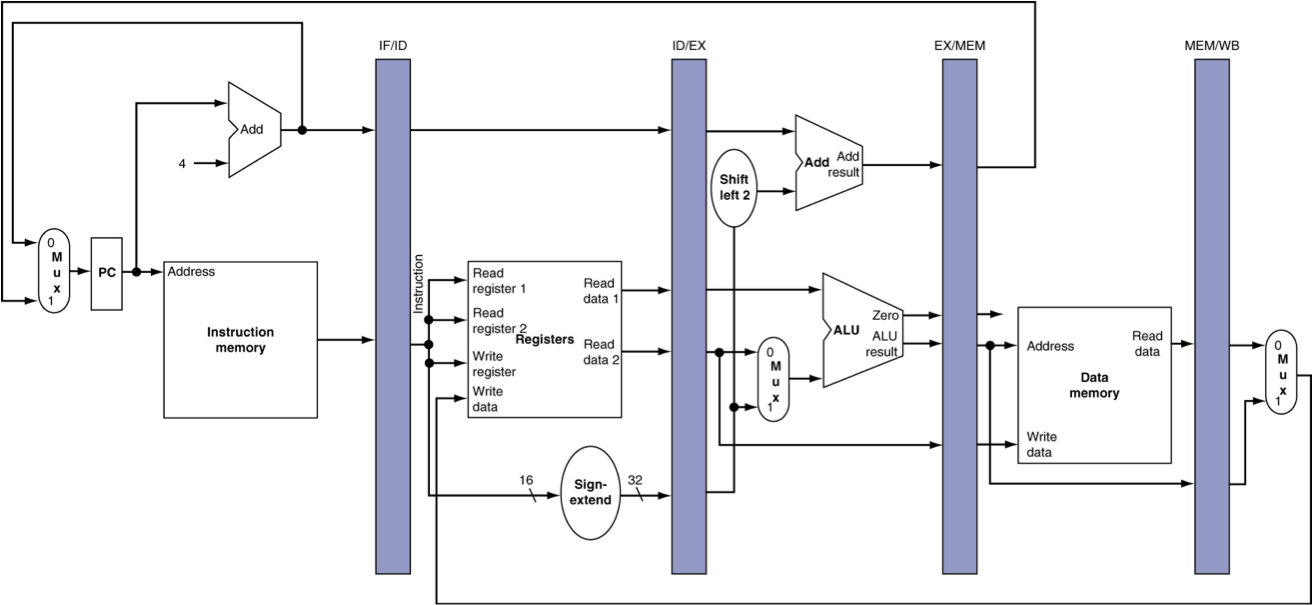
\includegraphics[width=0.8\textwidth]{1_introduction/img/MIPS_pipe.png}
\caption{MIPS pipeline \cite{John-L.-Hennessy:2009wq}}
\label{fig:mips_pipe}
\end{figure}

Introducing pipelining will generally lower the Clocks Per Instruction (CPI) rate of a processor to below 1.0. Special hardware has been developed, such as forwarding units, branch predictors, and speculative execution that will try to increase the CPI to a value that approaches 1.0. 

If a higher then 1.0 CPI is desired multiple instructions need to be executed during a single clock cycle. Machines that can execute multiple instructions are called multi issue machines. These types of processors use special hardware to find dependencies between instructions and to determine which instructions can be executed in parallel. These techniques include Tomasulo’s algorithm for Out of Order execution and register renaming. Most modern processors use these techniques to increase performance.

Finding dependencies between instructions becomes increasingly complex when the issue width of machines is increased. The Pentium 4 processor demonstrated the limitations of further ILP extraction in a spectacular way. It used a 20-stage pipeline \cite{John-L.-Hennessy:2012bs} with seven functional units. It operated on RISC-like micro-ops instead of x86 instructions and could handle 50 in-flight instructions at a time.

The amount of silicon and energy that was dedicated to finding and executing ILP made the Pentium 4 processor very inefficient. The expected clock frequency increase that Intel expected the hyper pipelined processor (6-7 GHz) to deliver never materialized and the Pentium 4 Netburst architecture was dropped for a much simpler architecture.

\cite{Wall:1993xy} showed the actual limitations of ILP extraction in hardware and demonstrated that other techniques need to be used to find and execute more ILP.

VLIW differs from multiple issue machines in that parallelism is found during compile-time instead of during run-time. This results in a processor that can be made significantly simpler because the ILP extraction algorithms do not need to be implemented and because dependency checking is not required during run-time. Additional ILP can also be found with the compiler because the compiler has got a higher level view of the code that is to be executed. Optimizations such as swing modulo scheduling and loop vectorization are nearly impossible to achieve in hardware because the higher level structure is no longer available. A compiler can interpret the higher level structure of a program and optimize the output for better scheduling.

The origins of the VEX ISA can be traced to the company Multiflow and John Fisher, one of the inventors of VLIW processors at Yale University \cite{Fisher:1983:VLI:1067651.801649}. Multiflow designed a computer that used VLIW processors to execute instructions up to 1024-bit in size. Along with these computers Multiflow also designed a compiler system that used trace based scheduling to extract ILP from programs. Reportedly the code base for the Multiflow compiler has been used in modern compiler such as Intel C Compiler (ICC) and HP VEX compiler because of the robustness and the amount of ILP that could be exposed by the compiler \cite{Lowney:1993qy}.

John Fisher has designed the VEX ISA as an example of VLIW type processors \cite{Joseph-A.-Fisher:2005cr}. His work includes the design of a VLIW processor and ISA and a compiler system that generates code for this processor.

Currently two different compilers exist that target the $\rho$-VEX processor: the VEX compiler and a GCC port developed by IBM. We will show that both existing compilers are not optimal and that a new compiler is required for the $\rho$-VEX project. Further we will present a LLVM based compiler that targets the $\rho$-VEX processor with performance and features similar to the VEX compiler. 

\section{Problem statement}
Currently, both the HP-VEX and GCC compilers can be used to generate code for the $\rho$-VEX processor. Both compilers have got a number of advantages and disadvantages that will be explored. The compilers will be judged on the following subjects: Code quality, support, languages support, backend supported and customization possibilities.
\newline

% \begin{itemize}
% 	\item \textbf{Code quality:}
% 	\item \textbf{Support:}
% 	\item \textbf{Front-end:}
% 	\item \textbf{Back-end:}
% 	\item \textbf{Customization:}
% \end{itemize}
HP-VEX:
\begin{itemize}
	\item \textbf{Code quality:} Excellent code quality and ILP extraction.
	\item \textbf{Support:} Bad, no active community.
	\item \textbf{Front-end:} Bad, only support for C.
	\item \textbf{Back-end:} Not applicable since compiler is specifically targeted to one architecture.
	\item \textbf{Customization:} Customization possible through machine description. Further research on optimization strategies not possible because compiler is proprietary and closed source. Because of this expanding the functionality of the compiler is impossible.
\end{itemize}

GCC:
\begin{itemize}
	\item \textbf{Code quality:} Excellent code quality with performance approaching that of commercial compilers (CITATION NEEDED).
	\item \textbf{Support:} There is a very active development community around GCC.
	\item \textbf{Front-end:} GCC supports a large number of programming languages including C, C++, Fortran and Java
	\item \textbf{Back-end:} Supoort exists for a large number of processors including x86, ARM, MIPS and ofcourse VEX
	\item \textbf{Customization:} Because GCC is open source the compiler can be customized to support new passes, optimizations and instructions.
\end{itemize}

Unfortunately GCC has a number of disadvantages that need mentioning.

\begin{itemize}
	\item \textbf{VEX code quality:} The VEX backend for GCC has not been optimized and the quality of the code is quite low. Performance of GCC executables is lower then code compiled by the HP-VEX compiler. Some programs do not function correclty when compiled by GCC. Some programs are unable to be compiled by GCC.
	\item \textbf{VEX reconfiguration:} The current GCC VEX compiler does not support run-time reconfiguration. The compiler has been set to a 4 issue width $\rho$-VEX and this cannot be changed without rebuilding GCC.	
	\item \textbf{Bloated:} GCC consists of millions of lines of code and is arguable one of the most complex programs in existence. This makes understanding GCC and developing for GCC very hard.
	\item \textbf{Complexity:} GCC is written in C. Design is complex, not very modular and documentation is not very good. Different parts of the compiler are linked in a complex way and it is very difficult to obtain a general picture on how the compiler operates. Because of the complexity it is difficult to achieve high performance in GCC.
\end{itemize}

The comparison shows that both the HP-VEX and GCC compilers have serious disadvantages. The fact that HP-VEX cannot be customized excludes it from further development for the $\rho$-VEX project. Bringing the GCC compiler performance and features up to the same level as HP-VEX will be very difficult because of the complexity involved with GCC development.  

In 2000 the LLVM project has been started with the goal of replacing the code generator in the GCC compiler. LLVM provides a modern, modular design and is written in C++. The GCC front-end was used to translate programs into LLVM compatibale intermediate representation. Around 2005 the Clang project was started which aimed to replace the GCC front-end with an independent front-end with support for C, C++ and ObjC. Currently the LLVM based compiler offers performance that approaches GCC but offering a significant improvement in terms of modularity, ease of development and "hackability". In addition the LLVM compiler can also be used to target different architectures such as GPU's and VLIW based processors.

\subsection{Goals}
The main goal of this thesis is to develop a new compiler for the $\rho$-VEX system. The compiler will be based on the LLVM compiler. The new compiler should have the following characteristics:

\begin{itemize}
	\item \textbf{Open source:} The compiler should be open source so the compiler can be customized and used for future research.
	\item \textbf{Code quality:} A new compiler should provide a significant improvement in terms of performance, code size and resource utilization.
	\item \textbf{Reconfigurability:} Charachteristics of the $\rho$-VEX processor should be reconfigurable during run-time.
\end{itemize}

\section{Methodology}
The following steps need to be completed for successful implementation of a $\rho$-VEX LLVM compiler.
\begin{itemize}
	\item Research $\rho$-VEX and VEX platform
	\item Research LLVM compiler framework
	\item Build LLVM based VEX compiler with following features:
	\begin{itemize}
		\item 4 issue width VLIW
		\item Code generation
		\item Assembly emitter
	\end{itemize}
	\item Add support for reconfigurability
		\begin{itemize}
			\item VEX machine description
			\item Reconfigure LLVM during runtime
		\end{itemize}	
	\item Optimize performance
	\begin{itemize}
		\item Instruction selection
		\item Hazard recognizer
		\item Register allocator
	\end{itemize}	
\end{itemize}




\section{Thesis overview}
The thesis is organized as follows. 
In Chapter \ref{chap:background} we will discuss the architecture of the $\rho$-VEX processor and the workings of the LLVM compiler suite. This chapter will demonstrate the supported instructions, run-time architecture, and show the general architecture of the $\rho$-VEX processor. The chapter will also show how the LLVM compiler operates and what steps are involved during compilation.

In Chapter \ref{chap:implementation} will discuss how the $\rho$-VEX compiler was implemented.  This chapter will present how a back-end is implemented in LLVM. We will show how code is transformed from the LLVM Intermediate Representation into a $\rho$-VEX specific assembly language. In addition we will also discuss new functionality that has been added to the LLVM compiler.

Chapter \ref{chap:optimization} will discuss how the performance of the LLVM compiler has been optimized. Problems that have been found are demonstrated and we will show how these problems have been solved to increase performance of the binaries.

Chapter \ref{chap:results} will explore the performance of the new compiler. Performance will be compared to existing compilers in terms of issue width, optimization levels and other metrics. A conclusion and recommendations for future research is presented in chapter \ref{chap:conclusion}.  


\acresetall

\chapter{Background}
\section{VEX System}
asd
\subsection{Architecture}
asd
\subsection{ISA}
asd
\subsection{Registers}
asd
\subsection{Run-time architecture}
asd

\section{LLVM Compiler infrastructure}
LLVM is based on the classic three-stage compiler architecture shown in figure \ref{fig:compiler_structure}. The compiler uses a number language specific front-ends, an optimizer and target specific backends. This modular design enables compiler designers to work on different parts of the compiler as a separate part. Support for a new processor can be added by building a new back-end. The existing front-end and optimizer can be reused for the new compiler.

\begin{figure}[ph!]
\centering
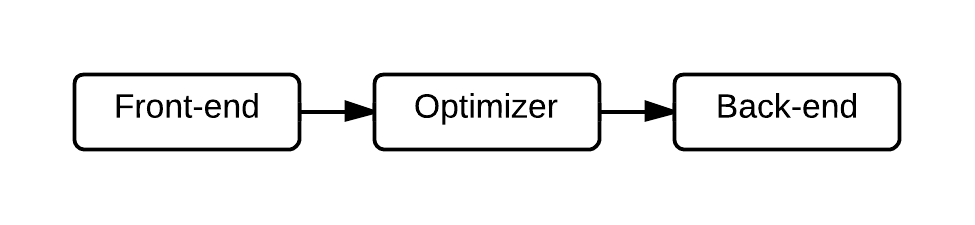
\includegraphics[width=0.8\textwidth]{2_background/img/Basic_compiler.png}
\caption{Basic compiler structure}
\label{fig:compiler_structure}
\end{figure}

The front-end is used to transform the plain text source code of a program into an intermediate representation that will be used during compilation process. This transformation is achieved by performing the following steps:

\begin{enumerate}
	\item \textbf{Lexical analysis:} Break input into individual tokens.
	\item \textbf{Syntax analysis:} Using a grammer the sequence of tokens is transformed into a parse tree which represents the structure of the program.
	\item \textbf{Semantic analysis:} Semantic information is added to the parse tree, type checking is performed and a symbol table is built.
\end{enumerate}

The resulting abstract syntax tree (AST) is transformed into LLVM IR and passed to the optimizer and backend of the compiler. These parts of the compilation process are completely language agnostic and do not require any other information from the front-end.

The optimizer is used to analyze and optimize the program. Optimization such as dead code elimination and copy propagation are performed during this phase but also more advanced operations that extract ILP (loop vectorization) can be enabled.

The back-end optimizes and generates code for a specific architecture. The LLVM IR is transformed into processor specific assembly instructions, allocates registers and schedules code for better performance.

\subsection{LLVM}
asd
\subsubsection{Front-end}
The modular design of LLVM enables the compiler to be used as a part of the existing GCC compiler. For example, the dragonegg GCC plugin is designed to replace the GCC code generator and optimizer with the LLVM backend. This would enable LLVM to be able to use the existing GCC based front-ends and supported languages.

Clang has been developed to allow LLVM to operate independently of GCC. Clang is a front-end supporting C, C++ and ObjC. The front-end is designed to be closely integrated with the Integrated Development Environment (IDE) allowing more expressive diagnostic messages. In addition Clang also aims to provide faster compilation and lower memory usage \cite{clang:features}.
\subsubsection{LLVM IR}
The front-end transforms a source code into the LLVM internal representation (LLVM IR). The LLVM IR is used to represent a high level language cleanly in a target independent way and is used during all phases of compilation. Instructions are similar to RISC instructions and can use three operands. Control flow instructions and type specific load/store instructions are used and an infinite amount of registers are available in Single Static Assignment (SSA) form. The LLVM IR is available as human readable text, in memory and in binary form \cite{llvm:presentation}.

The LLVM IR is designed to expose high-level information for further optimization. Examples of high-level information include dataflow through SSA form, control-flow graphs, language independent type information and explicit use of pointer arithmetic. 

Primitives such as voids, floats and integers are natively supported in the LLVM IR. The bitwidth of the integers can be defined manually. Pointers, arrays, structures and functions are derived from these basic types.

Object oriented constructs such as classes and virtual methods are not natively supported but can be built using the existing type system. For example a C++ class can be represented by a struct and a list of methods. 

The SSA based dataflow form allows the compiler to efficiently perform code optimizations such as dead code elimination and constant propagation. 

Figure \ref{lst:C_Example} shows an example program in C. The equivalent LLVM IR representation is shown in figure \ref{lst:LLVM_IR}.

\lstset{numbers=none, captionpos=b}
\begin{lstlisting}[language=C,caption={C example program},label=lst:C_Example]
int main() {
	int sum = 1;

	while(sum < 10)
	{
		sum = sum + 1;
	}
	return sum;
}
\end{lstlisting}


\lstset{numbers=none, captionpos=b}
\begin{lstlisting}[language=llvm,caption={LLVM Intermediate representation},label=lst:LLVM_IR]

define i32 @main() nounwind ssp uwtable {
  %1 = alloca i32, align 4
  %sum = alloca i32, align 4
  store i32 0, i32* %1
  store i32 1, i32* %sum, align 4
  br label %2

; <label>:2                                       ; preds = %5, %0
  %3 = load i32* %sum, align 4
  %4 = icmp slt i32 %3, 10
  br i1 %4, label %5, label %8

; <label>:5                                       ; preds = %2
  %6 = load i32* %sum, align 4
  %7 = add nsw i32 %6, 1
  store i32 %7, i32* %sum, align 4
  br label %2

; <label>:8                                       ; preds = %2
  %9 = load i32* %sum, align 4
  ret i32 %9
}

\end{lstlisting}

\subsubsection{Code generation}
During code generation the optimized LLVM IR is translated into machine specific assembly instructions. The modular design of LLVM enables generic algorithms to be used for this process. 

A backend is described in a domain specific language (DSL) called tablegen. The tablegen files describe properties of a backend such as available instructions, registers, calling convention and pipeline structure. During compilation of LLVM the tablegen files are converted into a C++ description of the backend. Tablegen has been specifically designed to describe the backend structure in a flexible and generic way. Common features can be more easily described using tablegen. For example the $Add$ and $Sub$ instruction are almost identical and using tablegen can be described in a more generic way. This results in less repetition and reduces the chance of error.

Because of the generic description of the backend large amount of code can be reused by each backend. Algorithms such as register allocation and instruction selection operate on the generic tablegen descriptions and do not require target specific hooks to operate correctly.
An additional advantage of this approach is that multiple algorithms are available to achieve certain functionality. For example, LLVM offers the developer a choice between four different register allocation algorithms. Each algorithm has a number of advantages and disadvantages and the developer can choose between an algorithm which matches the target processor best.

At the moment not all parts of the backend can be described in Tablegen and hand written C++ code is still needed for a backend to operate. As LLVM develops more parts of the backend description should be integrated into the backend. 

The following sequence is completed to translate LLVM IR into target specific assembly language:
\begin{enumerate}
\item Instruction selection
\item Scheduling
\item Register allocation
\item Prologue / epilogue insertion
\item Assembly printing
\end{enumerate}


\acresetall

\chapter{Implementation}
\label{chap:implementation}
The previous chapter demonstrated the architecture of the $\rho$-VEX processor and of the LLVM compiler. We have also shown that the LLVM compiler currently has support for a VLIW type processor. In this chapter we will show how the LLVM-based backend for the $\rho$-VEX processor has been implemented.

\section{Tablegen}
LLVM uses a domain-specific language (DSL) called \texttt{tablegen} to describe features of the backend such as instructions, registers, and pipeline information. 

\texttt{tablegen} uses a object-oriented approach to describe functionality. Information is described in classes and definitions that are called \emph{records}. Inheritance is supported so classes can derive information from superclasses. In addition, multiclasses can be used to instantiate multiple abstract records at once.

The \texttt{tablegen} tool aims to provide a flexible way to describe processor features. For example processor instructions could be described as follows:

A class is created that represents an abstract instruction. The class will describe information that is of direct importance to code generation such as opcode, register usage and immediate values but also information that is needed during the code generation such as liveness information, instruction pattern and scheduling information.

\begin{lstlisting}[language=tblgen]
class rvexInst<dag outs, dag ins, string asmstr, list<dag> pattern,
               InstrItinClass itin, Format f, CType type>: Instruction
{
}
\end{lstlisting}

The \texttt{rvexInst} class is used for all type of instructions that are supported by the $\rho$-VEX processor. Multiple instructions with common feature such as \texttt{add}, \texttt{sub}, and \texttt{and} can be described in subclasses that inherit from the \texttt{rvexInst} class. For example, the class \texttt{ArithLogicR} holds arithmetic instructions that use three register operands. The class describes common features such as the instruction string format and the instruction pattern that is used during instruction selection.

\begin{lstlisting}[language=tblgen]
class ArithLogicR<string instr_asm, SDNode OpNode,
                  InstrItinClass itin, RegisterClass RC, bit isComm = 0, CType type>:
  rvexInst <(outs RC:$ra), (ins RC:$rb, RC:$rc),
     !strconcat(instr_asm, "\t$ra = $rb, $rc"),
     [(set RC:$ra, (OpNode RC:$rb, RC:$rc))], itin, type> 
{
}
\end{lstlisting}

The following code shows how to define instructions that inherit from the \texttt{ArithLogicR} class. The instruction is defined as using the \texttt{ArithLogicR} class with certain parameters that match the instruction properties. These properties include instruction string, LLVM IR opcode, and other information that is needed during compilation.

\begin{lstlisting}[language=tblgen]
def ADD         : ArithLogicR<"add ", add, IIAlu, CPURegs, 1, TypeIIAlu>;
\end{lstlisting}

Figure \ref{fig:tblgen} displays an example of how individual instructions inherit from higher level classes. The final class is a \texttt{rvexInstr} that contains a description of all the available $\rho$-VEX instructions.

\begin{figure}[ht]
\centering
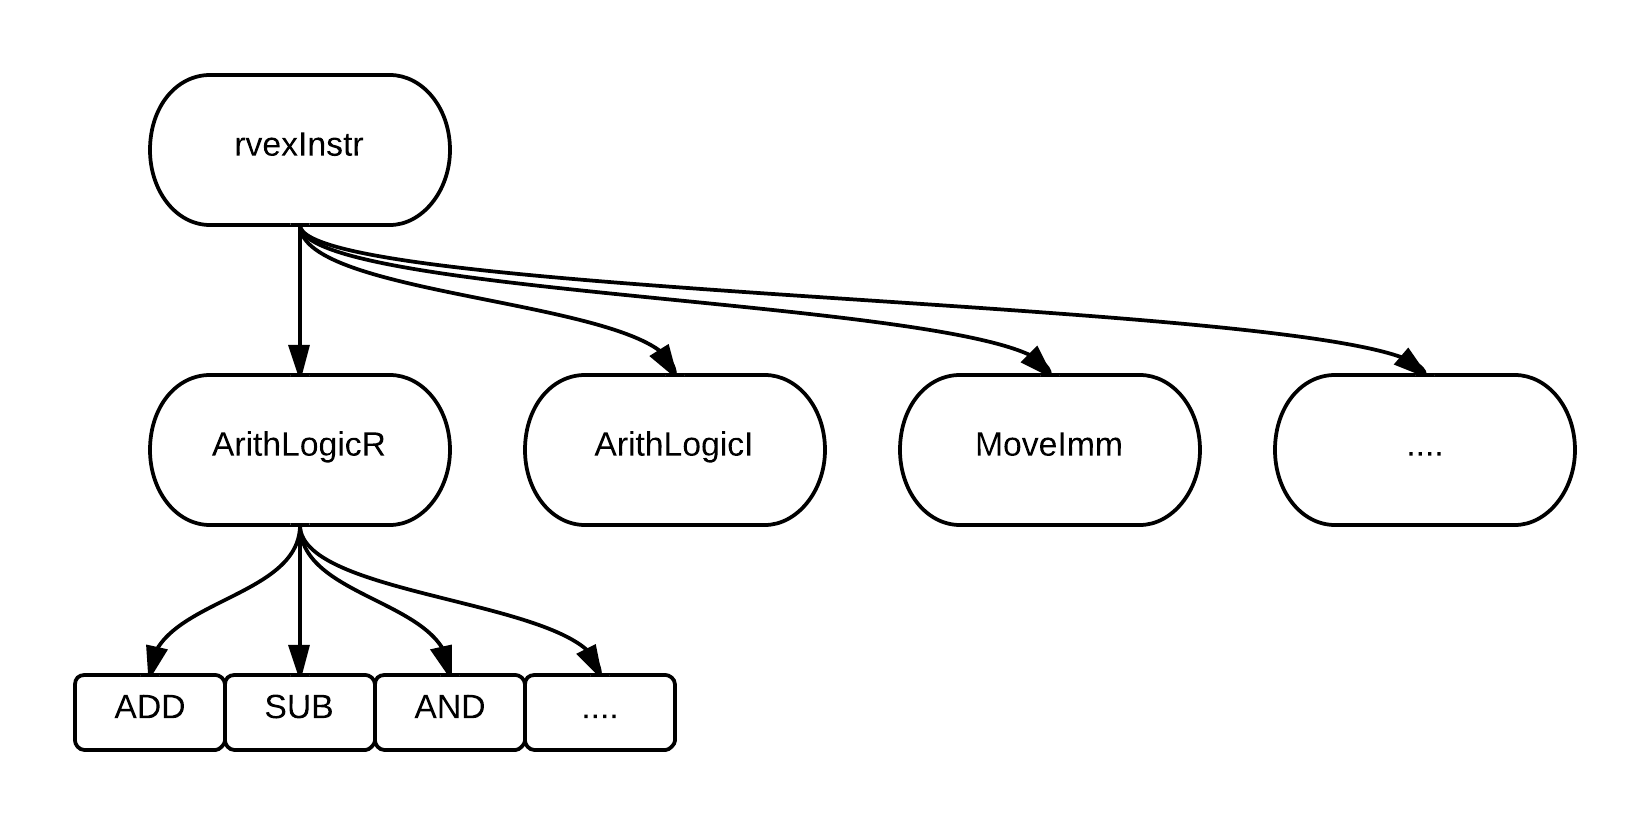
\includegraphics[width=0.8\textwidth]{3_implementation/img/instr.png}
\caption{\texttt{tblgen} instructions}
\label{fig:tblgen}
\end{figure}

\texttt{tablegen} provides for a very flexible way to describe backend functionality. The existing LLVM backends use \texttt{tablegen} in a variety of ways which best match the target processor. 

The \emph{tblgen} tool is used to transform the \texttt{tablegen} input files into C++. The resulting C++ files contain enums, structs and arrays that describe the properties. The instruction selection part is transformed into imperative code that is used by the backend for pattern matching. 

\subsection{Register definition}
LLVM uses a predefined class \texttt{register} to handle register classes. All $\rho$-VEX registers are derived from this empty class. The \texttt{rvexReg} class is used to define all type of $\rho$-VEX registers. 

\begin{lstlisting}[language=tblgen]
class rvexReg<string n> : Register<n> {
  field bits<7> Num;
  let Namespace = "rvex";
}
\end{lstlisting}

The \texttt{rvexReg} class is used to define the general purpose registers and the branch registers.
\begin{lstlisting}[language=tblgen]
class rvexGPRReg<bits<7> num, string n> : rvexReg<n> {
  let Num = num;
}

class rvexBRReg<bits<7> num, string n> : rvexReg<n> {
  let Num = num;
}
\end{lstlisting}

Each physical register is defined as an instance of one of these classes. For example, R5 is defined as follows. The register is associated with a register number, a register string, and a dwarf register number that is used for debugging.

\begin{lstlisting}[language=tblgen]
def R5 : rvexGPRReg< 5, "r0.5">, DwarfRegNum<[5]>;
\end{lstlisting}

The physical registers are divided in two register classes for the general purpose registers and for the branch registers. The register classes also define what type of value can be stored in the physical register.

\begin{lstlisting}[language=tblgen]
def CPURegs : RegisterClass<"rvex", [i32], 32, 
  (add
    (sequence "R%u", 0, 63),
    LR, PC
  )>;

def BRRegs   : RegisterClass<"rvex", [i32], 32, 
  (add 
    (sequence "B%u", 0, 7)
  )>;
\end{lstlisting}

The branch registers have been defined to also use 32 bit values even though in reality the branch register is only 1 bit wide. This has been done because LLVM had a lot of trouble identifying the correct instruction patterns for compare instructions. The $\rho$-VEX compare instruction can produce results in both the CPURegs and the BRegs as illustrated in the following example:

\begin{lstlisting}
<1 bit>BRRegs = Operation, <32 bit>CPURegs, <32 bit>CPURegs
<32 bit>CPURegs = Operation, <32 bit>CPURegs, <32 bit>CPURegs
\end{lstlisting}

The LLVM compiler is unaware that when the compare instruction is used to define a 32-bit result only the lowest bit will be set. The compiler tried to resolve this issue by inserting \texttt{truncate} and \texttt{zero\_extend} instructions even though this is not required. This has been solved by implementing the BRRegs as 32 bit wide so LLVM will not insert truncate and extend instructions when operating on these type of instructions.

\subsection{Pipeline definition}
\texttt{tablegen} can be used to describe the architecture of the processor in a generic way. LLVM will schedule an instruction to a processor functional unit during the scheduling pass. The following code describes the available functional units for a 4-issue a $\rho$-VEX processor.

\begin{lstlisting}[language=tblgen]
def P0 : FuncUnit;
def P1 : FuncUnit;
def P2 : FuncUnit;
def P3 : FuncUnit;
\end{lstlisting}

Each instruction is associated with an instruction itinerary. An instruction itinerary is used to group scheduling properties of instructions together. The $\rho$-VEX processor uses the following instruction itineraries.

\begin{lstlisting}[language=tblgen]
def IIAlu              : InstrItinClass;
def IILoadStore        : InstrItinClass;
def IIBranch           : InstrItinClass;
def IIMul              : InstrItinClass;
\end{lstlisting}

The functional units and instruction itineraries are used to describe the properties of the $\rho$-VEX pipeline. The scheduling properties are derived from a description of an instruction stage with certain properties and the associated instruction itinerary. These properties include the \emph{cycle count}, that describes the length of the instruction stage, and the functional units that can execute the instruction. The following itinerary describes a $\rho$-VEX pipeline with four functional units. Each functional unit is able to execute every instruction except for load / store instructions. Only \texttt{P0} is able to execute load / store instructions. These instructions take two cycles to complete.

\begin{lstlisting}[language=tblgen]
def rvexGenericItineraries : ProcessorItineraries<[P0, P1, P2, P3], [], [
  InstrItinData<IIAlu              , [InstrStage<1,  [P0, P1, P2, P3]>]>,
  InstrItinData<IILoadStore        , [InstrStage<2,  [P0]>]>,
  InstrItinData<IIBranch           , [InstrStage<1,  [P0, P1, P2, P3]>]>,
  InstrItinData<IIIMul             , [InstrStage<1,  [P0, P1, P2, P3]>]>,
]>;
\end{lstlisting}

The machine model class is used to encapsulate the processor itineraries and certain high-level properties such as issue width and latencies.

\begin{lstlisting}[language=tblgen]
def rvexModel : SchedMachineModel {
  let IssueWidth = 2;
  let Itineraries = rvexGenericItineraries;
}
\end{lstlisting}

\subsection{Other specifications}
\texttt{tablegen} is also used to describe other properties of the target processor. LLVM has stated as goal to move more parts of the backend description to the \texttt{tablegen} format because \texttt{tablegen} offers such a flexible implementation. At the moment \texttt{tablegen} is also used to implement:

\begin{itemize}
  \item Calling convention
  \item Subtarget features
\end{itemize}

\section{Code generation}
To understand how the compiler changes code from the LLVM IR representation to VEX assembly instruction it is necessary to understand how the code generation process works. The code generation process is divided into multiple steps, called passes, which are performed in order. 

\subsection{Instruction transformation}
The instruction selection phase is completed in the following steps
\begin{itemize}
  \item \textbf{Build initial DAG:} Transform the LLVM IR into a DAG that contains illegal types and instructions. The initial DAG is a one-to-one representation of the LLVM IR code.
  \item \textbf{Legalize instructions:} Illegal instructions are expanded and replaced with legal instructions.
  \item \textbf{Legalize types:} Transform the types used in the DAG to types that are supported by the target processor 
  \item \textbf{Instruction selection:} The legalized DAG still contains only LLVM IR instructions. The DAG is transformed to a DAG containing target-specific processor instructions.
\end{itemize}

\subsection{Instruction Lowering}
The \texttt{rvexISelLowering} class gives a high-level description of the operations that are supported by the target processor. The class can describe how the compiler should handle each LLVM IR instruction using four parameters: Legal, Expand, Promote or Custom. The default option is Legal, which implies that the LLVM IR instruction is natively supported by the target processor.

\subsubsection{Expanded instructions}
The Expand flag is used to indicate that the compiler should try to expand the instruction into simpler instructions. 
For example consider the LLVM IR \texttt{UMUL\_LOHI} instruction. This instruction multiplies two values of type \texttt{iN} and returns a result of type \texttt{i[2*N]}. Through expansion this instruction will be transformed into two mult instructions that calculate the low part and the high part separately.

\begin{lstlisting}[language=c] 
setOperationAction(ISD::UMUL_LOHI,  MVT::i32, Expand);
\end{lstlisting}

\subsubsection{Promote instruction}
Some instruction types are not natively supported and the type should be promoted to a larger type that is supported by the target processor. This feature is useful for supporting logical operations on Boolean functions. The following operation transforms an AND instruction that operates on a boolean value to a larger type.

\begin{lstlisting}[language=c] 
setOperationAction(ISD::AND,        MVT::i1, Promote);
\end{lstlisting}

\subsubsection{Custom expansion}
There are some instructions that cannot be expanded automatically by the compiler. To support these instructions the instruction expansion can be defined manually. For example consider the MULHS instruction that multiplies two numbers and returns the high part.

\begin{lstlisting}[language=c] 
setOperationAction(ISD::MULHS,      MVT::i32, Custom);
\end{lstlisting}

When a MULHS instruction is parsed the compiler will execute a function that describes the sequence of operations to lower this instruction. This sequence of instructions is implemented in the \texttt{LowerMULHS} function of the \texttt{rvexISelLowering} class. The \texttt{LowerMULHS} function is used to manually traverse the DAG and insert a sequence of instructions to support the operation.

For each instruction that requires custom lowering a \texttt{LowerXX} function has been defined.

\subsection{Instruction selection}
After instruction lowering the DAG contains LLVM IR operations and types that are all supported by the target processor but the DAG still contains only LLVM IR operations and no target-specific operations. The \texttt{rvexISelDAGToDag} class is used to match LLVM IR instructions to instructions of the target processor. The bulk of this class is generated automatically from the \texttt{tablegen} description but instructions can also be matched manually.

\subsection{New instructions}
The $\rho$-VEX processor supports some instructions that have no equivalent LLVM ISD operation. These instructions include \texttt{divs}, \texttt{addcg}, \texttt{min}, \texttt{max}, and others. Two stages are required to add support for these operations:

\begin{enumerate}
  \item \textbf{Extend ISD namespace:} The new instructions will be added to the ISD namespace. This means that the LLVM IR will be \emph{extended} with the new instructions.
  \item \textbf{Instruction lowering:} Describe when these instruction should be inserted in the LLVM IR. For example, lowering of the LLVM IR \texttt{div} instruction uses a custom lowering function to describe the algorithm that uses the $\rho$-VEX \texttt{divs} instruction.
  \item \textbf{Instruction matching:} New pattern matching rules need to be defined that map a custom instruction from the extended ISD namespace to the final target-specific $\rho$-VEX instructions.
\end{enumerate}

For this example we are going to consider the $\rho$-VEX \texttt{divs} instruction.

\subsubsection{Extend ISD namespace}
The ISD namespace can be extended with target-specific operations by defining the instruction type and the instruction name. Because the \texttt{divs} instruction uses five operands a custom instruction type will be used. The following code shows the definition for the custom instruction type. This type describes an instruction that produces two results and consumes three operands.

\begin{lstlisting}[language=tblgen]
def SDT_rvexDivs          : SDTypeProfile<2, 3
                                          [SDTCisSameAs<0, 2>,
                                          SDTCisSameAs<0, 3>,
                                          SDTCisInt<0>, SDTCisVT<0, i32>,
                                          SDTCisSameAs<1,4>,
                                          SDTCisInt<1>, SDTCisVT<1, i1>]>;
\end{lstlisting}

The next step involves defining the name of the custom instruction. The instruction is defined as a custom \texttt{SDNode} and uses the instruction type that has been defined earlier. This operation expands the LLVM ISD namespace with custom operations that are only available in the $\rho$-VEX backend.

\begin{lstlisting}[language=tblgen]
def rvexDivs              : SDNode<"rvexISD::Divs", SDT_rvexAddc>;
\end{lstlisting}

\subsubsection{Instruction lowering}
The \texttt{rvexISelLowering} class is extended with functions that produce the new ISD operation. For this example LLVM IR \texttt{div} instruction is custom lowered in the \texttt{LowerDIVS} function. In this function an algorithm is implemented that uses the new \texttt{divs} SDNode.

After instruction lowering a DAG will have been produced that contains only legal ISD operations and the new ISD operations that have been defined earlier.

\subsubsection{Instruction selection}
The following code describes the instruction class that is used by the \texttt{divs} instruction. This class describes the instruction string, register class properties and certain scheduling properties of this instruction. Note that the instruction pattern is empty because the current version of \texttt{tablegen} has no support for instructions that produce multiple results. A custom pattern matching function will need to be implemented in the \texttt{rvexISelDAGToDAG} class.

\begin{lstlisting}[language=tblgen]
class ArithLogicC<bits<8> op, string instr_asm, SDNode OpNode,
                  InstrItinClass itin, RegisterClass RC, RegisterClass BRRegs, bit isComm = 0, CType type>:
  FA<op, (outs RC:$ra, BRRegs:$co), (ins RC:$rb, RC:$rc, BRRegs:$ci),
     !strconcat(instr_asm, "\t$ra, $co = $rb, $rc, $ci"),
     [], itin, type> {        // Note empty instruction matching pattern
  let shamt = 0;
  let isCommutable = isComm;  // e.g. add rb rc =  add rc rb
  let isReMaterializable = 1;
}
\end{lstlisting}

The last step is to define the properties of the custom instruction.

\begin{lstlisting}[language=tblgen]
def rvexDIVS    : ArithLogicC<0x13, "divs ", rvexDivs, IIAlu, CPURegs, BRRegs, 1, TypeIIAlu>;
\end{lstlisting}

The \texttt{rvexISelDAGToDAG} class is used to define the custom instruction selection patterns. This class implements the pattern matching code that is generated from the \texttt{tablegen} description files. The class has a separate \texttt{select} function to match instructions that have no pattern matching rules defined.

The select function uses switch statements to select between custom \texttt{SDNodes}. The following function implements the pattern matching rule for the \texttt{divs} instruction that replaces the extended ISD \texttt{divs} instruction with the $\rho$-VEX instruction \texttt{rvexDIVS}. The \texttt{rvexDIVS} instruction has been defined earlier in the \texttt{tablegen} description files.

\begin{lstlisting}[language=C++]   
  case rvexISD::Divs: {
    SDValue LHS = Node->getOperand(0);
    SDValue RHS = Node->getOperand(1);
    SDValue Cin = Node->getOperand(2);
    return CurDAG->getMachineNode(rvex::rvexDIVS, dl, MVT::i32, MVT::i32,
                                  LHS, RHS, Cin);
    break;
  }
\end{lstlisting}

\subsubsection{Other cases}
Some $\rho$-VEX-specific instructions, such as the SHXADD instructions, are easier to support and do not need custom lowering. These instructions are also defined with empty pattern matching rules so the compiler will never insert them automatically. However the SHXADD instruction is easier to support because we can also match an instruction to a sequence of instructions. The following code describes a rule to replace the sequence \texttt{ADD (LHS\textless\textless1), RHS} with \texttt{SH1ADD LHS, RHS}.

\begin{lstlisting}[language=tblgen]
def : Pat<(add (shl CPURegs:$lhs, (i32 1)), CPURegs:$rhs),
          (SH1ADD CPURegs:$lhs, CPURegs:$rhs)>;
\end{lstlisting}

\subsection{Floating-point operations}
$\rho$-VEX processor does not natively support floating-point instructions. Instead software functions are used to execute FP operations. During instruction lowering FP operations are translated into library calls that will execute the instructions.

The LLVM compiler uses library functions that are compatible with the GCC Soft-FP library. The LLVM compiler-RT library is compatible with the GCC soft-FP library and is used for execution of FP instructions. Compiler-RT is a runtime library developed for LLVM that provides for these library functions.

\subsection{Scheduling}
During the scheduling pass the \texttt{SDNodes} are transformed into a sequential list form. Different schedulers are available for different processor types. For instance the register pressure scheduler will always try to keep the register pressure minimal which works better for x86 type processors. For the $\rho$-VEX processor a VLIW scheduler is used.

The list still does not contain valid assembly instructions. Virtual SSA based registers are still used and all the stack references do not reference true offsets.

\subsection{Register allocation}
During register allocation the virtual registers are mapped to available physical registers of the target processor. The register allocator considers the calling convention, reserved registers and special hardware registers during allocation. In addition the register allocator also inserts spill code when a register mapping is not available.

Liveness analysis is used to determine which virtual registers are used at a certain time. The liveness of virtual registers can be determined easily through the SSA based form of the input list. Multiple register allocation algorithms are available. All algorithms operate on the liveness information.

\subsection{Hazard recognizer}
The $\rho$-VEX processor has no way to recognize hazards or halt execution of code for a cycle. Because of this the correct scheduling of instructions is important for correct execution. Consider the following sequence of code:

\begin{lstlisting}[language=rvex]
  ldw $r0.2 = 0[$r0.2]  # Load from main memory
;;
  add $r0.2 = $r0.2, 2  # Add 2 to register
;;
\end{lstlisting}

After execution the register r0.2 will contain an undefined value because the load instruction has not completed execution. The compiler needs to insert an instruction or nop between the load and add instruction for correct execution. The correct instruction sequence should be the following:

\begin{lstlisting}[language=rvex]
  ldw $r0.2 = 0[$r0.2]  ## Load from main memory
;;
                        ## Empty instruction
;;
  add $r0.2 = $r0.2, 2  ## Add 2 to register
;;
\end{lstlisting}

The \texttt{ScheduleHazardRecognizer} is only able to resolve structural hazards, not data hazards. In Chapter \ref{chap:optimization} we will describe how the hazard recognizer has been combined with a new scheduling algorithm to resolve both data and structural hazards.

\subsection{Prologue and epilogue insertion}
After the register allocation pass the prologue en epilogue functions can be inserted. The prologue and epilogue pass is used to calculate the correct stack offset for each variable. Code is inserted that reserves room on the stack and saves / loads variables from the stackframe.

\subsection{VLIW Packetizer}
The packetizer pass is an optional pass that is used for VLIW targets. The packetizer receives a list of sequential machine instructions that need to be bundled for VLIW processors. 

The \texttt{tablegen} pipeline definition is used to build a DFA that represents the resource usage of the processor. The DFA can be used to determine to which functional unit an instruction can be mapped and if enough functional units are available.

The DFA representation is powerful enough to consider different properties of functional units. For example consider a 4-issue width VLIW processor but with only one unit supporting load / store operations. The DFA can model this pipeline and guarantee only one load / store instruction will be executed per clock cycle.

The VLIW packetizer also checks if certain instructions are legal to bundle together. The packetizer can be customized to check for hazards such as data dependency hazards, anti dependencies and output dependencies. Custom hazards can also be inserted to make sure that control flow instructions are always in a single bundle.

\section{New LLVM features}
This section describes features that have been added to the LLVM compiler. Currently, the $\rho$-VEX backend is the only backend that supports these kind of features.

\subsection{Generic binary support}
% FIXME uitleggen hoe instructies worden geserialized

By disallowing RAW hazards in instruction bundles, binaries can be generated that can execute on any $\rho$-VEX processor irrespective of issue width. For example consider the following instruction packet. The RAW hazard will occur on the r0.8 register.

\begin{lstlisting}[language=rvex]
  add $r0.10  = $r0.10, $r0.11
  add $r0.12  = $r0.12, $r0.13
  add $r0.14  = $r0.14, $r0.8
  add $r0.8   = $r0.8, $r0.9
;; 
\end{lstlisting}

Execution of this code on a 4-issue width processor will be fine but if this instruction is executed on a 2-issue width processor a problem will arise. The contents of register r0.8 will be changed during execution of the first bundle and execution of the second bundle will produce an invalid result.

This bundle should be split into two instructions during compilation. This can be achieved by checking for RAW hazards inside a bundle during the VLIW packetizer pass. The VLIW packetizer will detect these hazards and split the instructions into different bundles so correct execution is guaranteed.

\subsection{Compiler parameterization}
The HP VEX compiler supports a machine description file that describes properties of the processor. Using this machine description certain parameters, such as issue width, multiply units, load / store units, and branch units can be customized. 

Currently the LLVM compiler supports parameterization through subtarget support. Backend features can be enabled and disabled with command line parameters. The ARM backend uses this approach to select between different ARMv7 architectures, floating point support and div/mul support. This approach would not be useful for the $\rho$-VEX processor because of the amount of features that can be customized. Each customizable feature would need a new subtarget. For example, when four features can be customized (W, X, Y and Z), then $W*X*Y*Z$ subtargets would be needed. Clearly, this approach is not usable for the $\rho$-VEX processor where multiple parameters can be customized with a wide range of possibilities.

A different approach is used that changes the target description during runtime of the compiler. The target processor features are described in the \texttt{rvexMCTargetDesc} class. During runtime a machine description file will be read parsed and information from this machine description will be used to update the \texttt{rvexMCTargetDesc} class. 

The following properties can be customized through the machine description file:

\begin{itemize}
  \item \textbf{Generic binary:} disable RAW hazard check in VLIW packetizer
  \item \textbf{Width:} issue width of the processor
  \item \textbf{Stages:} describes all the available functional units an the amount of cycles an instruction fills a functional unit.
  \item \textbf{Instruction itinerary:} maps an instruction itinerary to a function unit. Also describes at what cycle the output contains a legal value.
\end{itemize}

The parameters are also used to generate the DFA that will track the resource usage. During the translation of the \texttt{tablegen} file an algorithm is used to generate a DFA from the available functional units. This algorithm has been implemented in the \texttt{rvexMCTargetDesc} class.

The location of the machine description file is passed to the \texttt{rvexMCTargetDesc} through command line parameters. Custom command-line parameters can be implemented in LLVM using \texttt{cl::opt} templates.

Some parameters such as the toggling of generic binary support is not handled through the \texttt{rvexMCTargetDesc} file. These parameters are used to set global state flags that can be read at anypoint in the compilation process. The \texttt{Is\_Generic\_flag} is used during the \texttt{rvexVLIWPacketizer} pass and during the liveliness calculation pass.

The following code demonstrates the configuration file for a 4-issue width  $\rho$-VEX processor with support for generic binaries. The \texttt{Stages} parameter uses three values. The first value describes the amount of clock cycles a instruction occupies a functional unit the second parameter is a bitmask for which functional unit can handle this instruction. The third parameter is currently not used.

The \texttt{InstrItinerary} parameter describes which type of instruction maps to which \texttt{Stage}. The first value describes which Stage an instruction is going to use, the second parameter describes when the result of the operation is available.

\begin{lstlisting}[language=config]
Generic         = 1;
Width           = 4; 
Stages          = {1, 15, 1}, {1, 1, 1}, {2, 2, 1};
InstrItinerary  = {1, 2}, {1, 2}, {3, 5}, {2, 3}, {1, 2}, {1, 2};
\end{lstlisting}

The compiler parameterization feature can be easily ported to other LLVM backends. The only part that has changed is the \texttt{rvexMCTargetDesc} class. 

\section{Conclusion}
In this section, we have shown how the $\rho$-VEX backend for the LLVM compiler has been implemented. Using the \texttt{tablegen} description we have described all the instructions that are supported by the $\rho$-VEX processor. We have also shown how LLVM IR code is transformed into a DAG that represents the original program. Through lowering functions this DAG is transformed into a DAG that contains only operations that are supported by the target processor. With instruction selection the DAG is transformed into a new DAG that contains target specific operations.

The finished DAG is transformed into a sequential list of instructions. This instruction list is used for the remaining passes. The remaining passes are used to map virtual registers to physical registers, emit prologue and epilogue functions and to perform VLIW packetization.

Support for floating-point operations has been added by porting the LLVM floating point library to the $\rho$-VEX processor.

Certain features that are required for the $\rho$-VEX processor were not available in the LLVM compiler. Features such as a machine description file are new to LLVM and we have shown what changes have been made to the LLVM compiler to support machine description files. In addition, we have shown how the backend has been updated to provide support for the $\rho$-VEX generic binary format.


\acresetall


\chapter{Optimization}
\label{chap:optimization}
The previous chapter described how the basic $\rho$-VEX LLVM compiler has been implemented. In this chapter we are going to discuss certain optimizations to improve the performance of binaries that are generated with the LLVM-based compiler.

\section{Machine scheduler}
% FIXME data-hazards?
A Machine Instruction scheduler is used to resolve structural and data hazards. The hazard recognizer that has been described earlier only resolves structural hazards. This means that the hazard recognizer can keep track of the functional units but it cannot keep track of data hazards between packets. The machine scheduler operates before the register allocator and is used to determine register allocation costs of each virtual register. This information is used during the register allocation pass to select a better mapping of physical to virtual registers that avoids expensive spills for commonly used virtual registers.

The Hexagon Machine scheduler has been customized to provide support for the $\rho$-VEX processor. The original Hexagon Machine Scheduler was used to perform packetization and to provide register allocation hints to the register allocator. The $\rho$-VEX machine scheduler has been enhanced with support for resolving data and structural hazards. 

The machine scheduler pass uses the VLIW packetization information to build temporary instruction packets. A register allocation cost metric is used to determine an optimal scheduling and packetization of instructions. The following $\rho$-VEX instructions can produce data hazards that need to be resolved with the machine scheduler:

\begin{itemize}
  \item \textbf{Multiply instructions:} 2 cycles
  \item \textbf{Load instructions:} 2 cycles
  \item \textbf{LR producing instructions:} 2 cycles
  \item \textbf{Compare and branch operations:} 2 cycles
\end{itemize}

The machine scheduler operates in two phases: building of an instruction queue and scheduling of the instruction queue.
During initialization of the machine scheduler two queues are built: The pending instruction queue and the available instruction queue. The available queue contains all the instructions that are available to schedule before a structural hazard occurs. The scheduler will schedule instructions until the available queue is empty and checks for any remaining structural hazards. If this hazard exists, a \texttt{nop} instruction will be inserted, otherwise nothing will be done. The machine scheduler will then load new instruction from the pending queue to the available queue until a new structural hazard occurs.

The scheduling phase is used to keep track of data hazards in instruction packets. The algorithm builds temporary packets and checks for data dependencies between each packet. If a data dependency has been found a \texttt{nop} instruction is inserted to resolve the hazard. Listing \ref{lst:scheduler} displays the algorithm in pseudo-code that is used to determine data dependencies. 


\begin{lstlisting}[language=python,label=lst:scheduler]
  # Get instruction from queue
  Candidate = GetCandidate(Available_Queue)

  if (!Candidate)
    # No Candidate found, structural hazard
    ScheduleMI(NULL, isNooped = True)

  # Check latencies for all predecessors of candidate
  for Predecessor in Candidate.Predecessors
    # Get instruction latency and scheduled cycle
    Latency     = Predecessor.Latency
    SchedCycle  = Predecessor.SchedCycle   

    if (Latency + SchedCycle > CurrentCycle)
      # Only 1 Noop per <def> of instruction
      if (Predecessor.Nooped == false)
        # Schedule Noop
        InsertNoop = True

        #                   
        Predecessor.Nooped = True
        Predecessor.SchedCycle--          

  # Add Candidate to current packet
  Reserve(Candidate)                       

  If (Packet.full)
    # If packet is full increase scheduling cycle
    CurrentCycle++;                        
    Packet.clear                           

  # Schedule instruction with Noop if required     
  Schedule(Candidate, InsertNoop)           

\end{lstlisting}

The $\rho$-VEX processor has a 1 cycle delay between defining a branch register and using a branch register. The scheduler has been customized to insert \texttt{nop} instruction proceeding each branch instruction. This solution is not optimal because the empty instruction could also be used to execute an instruction that is independent. Unfortunately, this proved impossible to implement in the current version of the LLVM compiler because branch instructions are not scheduled with the machine scheduler. The machine scheduler uses branch instructions as scheduling boundaries and does not include these instructions in the temporary instruction packets. During VLIW packetization branch instructions are packed as single instructions that are not executed concurrently with other operations.

The following instruction sequence illustrates the current solution: 
% FIXME layout
\newpage

\begin{lstlisting}[language=rvex]
  c0  cmpgt   $b0.0, $r0.2, 9
;;

;;
  c0  br    $b0.0, .BB0_3
;;
\end{lstlisting}

The following code uses select instruction instead of branch instruction and does not need the 1 cycle delay between instructions. Select instructions are arithmetic type instructions.

\begin{lstlisting}[language=rvex]
  c0  cmpgt   $b0.0, $r0.2, 9
;;
  c0  slct    $r0.1 = $b0.0, $r0.2, $r0.3 
;;
\end{lstlisting}

After the machine scheduler pass the temporary instruction bundles are deleted but the instruction ordering remains. Between the machine scheduler and VLIW packetization the only pass that can insert new code is the register allocator when spill code is introduced. During the \texttt{ExpendPredSpill} pass the spill code is checked for data dependencies and additional \texttt{nops} are inserted when required.

The final packetization occurs during the VLIW packetizer pass. The VLIW packetizer detects \texttt{nop} operations and outputs these instructions as \emph{barrier} packets. These packets do not contain any instructions.

% Moet ik dit hier vermelden of is dit beter om uit te lichten bij future work
Scheduling could be improved further by integrating the instruction scheduling with the register allocation. The \texttt{getCandidate} function should be expanded to take into account both register pressure and resource utilization. In \cite{Bradlee:1991:IRA:106973.106986} an approach is discussed that minimizes register pressure and resource usage and can optimize performance.

\section{Branch analysis}
Analysis of assembly files generated with the LLVM-based compiler showed that branches were not handled correctly. Consider the following C code:

\begin{lstlisting}[language=c]
  if (c)
    return 1;
  else
    return 2;
\end{lstlisting}
% FIXME layout
\newpage
This code will be roughly translated into the following assembly code:


\begin{lstlisting}[language=rvex]
  br    $b0.0, .BB0_2
;;
  goto  .BB0_1            ## Goto not required
;;
.BB0_1
  add $r0.3   = $r0.0, 1
;;
  goto  .BB0_3
;;
.BB0_2
  add $r0.3   = $r0.0, 2
;;
.BB0_3
  return
;;
\end{lstlisting}

The first \texttt{goto} operation is not required because it will jump to an adjacent block of instructions. A branch analysis pass has been developed that can recognize jumps to adjacent blocks and remove unnecessary \texttt{goto} instructions. This pass works by iterating over each \texttt{MachineBasicBlock} and finding \texttt{MachineInstr} that are branch instructions. If a branch instruction is found the instruction is analyzed to determine if the \texttt{goto} statements can be removed. 

In addition, LLVM hooks for \texttt{insertbranch}, \texttt{removebranch}, and \texttt{ ReverseBranchCondition} have been implemented that allow the BranchFolding pass to further optimize branches.


\section{Generic binary optimization}
Research \cite{Anthony-Brandon:2013jk} has shown  that generic binaries incur a performance penalty because of inefficient register usage. Consider the previous generic binary example again:

\begin{lstlisting}[language=rvex]
  add $r0.10  = $r0.10, $r0.11
  add $r0.12  = $r0.12, $r0.13
  add $r0.14  = $r0.14, $r0.8
  add $r0.8   = $r0.8, $r0.9
;; 
\end{lstlisting}

This instruction packet is not legal because of the RAW hazard that is caused by \texttt{r0.8}. The current approach to fix the RAW hazard is to split the instruction packet into two separate instructions. 

\begin{lstlisting}[language=rvex]
  add $r0.10  = $r0.10, $r0.11
  add $r0.12  = $r0.12, $r0.13
  add $r0.14  = $r0.14, $r0.8
;;
  add $r0.8   = $r0.8, $r0.9
;;
\end{lstlisting}

Because more instruction packets are used than required the amount of ILP that is extracted decreases and the performance of the resulting binary decreases. Performance could be improved by using a different register for the last assignment of \texttt{r0.8}. 

\subsection{Problem statement}
This kind of optimization poses a significant challenge for VLIW type compilers because the register allocation pass is executed before the VLIW packetization. This implies that the register allocator has no information about which operations will be grouped together and for which operations an extra register should be used.

A solution could be to perform VLIW packetization before register allocation is completed. This would allow the register allocation pass to determine if a RAW hazard occurs inside a packet and to assign an extra register if needed.

In practice this approach is not possible because between the register allocation pass and the VLIW packetizer pass other passes are run that can change the final code. For example, the register allocator pass can insert spill code and the prologue / epilogue insertion pass inserts code related to the stack layout. Inserting new instructions into instructions packets that have already been formed is very ugly because \emph{packet spilling} could occur where a packet that is already full needs to move instructions to the next packet, etc. 

The new machine scheduler could be customized to retain bundling information for the register allocator. Due to the complexity of implementing this approach we have chosen to change the register allocator itself and to make register allocation less aggressive. 

The liveliness allocation pass determines when a virtual register is used. The register allocator uses this information to create a register mapping with minimal register pressure.

By increasing the live range of a virtual register it should be possible to force the register allocator to use more registers when multiple virtual registers are used consecutively. Consider again the previous example:

\begin{lstlisting}[language=rvex]
  add $r0.10  = $r0.10, $r0.11
  add $r0.12  = $r0.12, $r0.13
  add $r0.14  = $r0.14, $r0.8
  add $r0.8   = $r0.8, $r0.9
;;
\end{lstlisting}

This would be transformed into the following code where the final \texttt{r0.8} assignment is changed to an unused register. 

\begin{lstlisting}[language=rvex]
  add $r0.10  = $r0.10, $r0.11
  add $r0.12  = $r0.12, $r0.13
  add $r0.14  = $r0.14, $r0.8
  add $r0.15  = $r0.8, $r0.9
;;
\end{lstlisting}

\subsection{Implementation} % (fold)
\label{sub:implementation}
The \texttt{LiveIntervals} pass is used to determine the live ranges of each virtual register. The pass uses the \texttt{LiveRangeCalc} class.
Each virtual register has an associated \texttt{SlotIndex} which tracks when the register becomes live and when the register is killed. The \texttt{SlotIndex} class also provides method that give information on the \texttt{MachineBasicBlock} (MBB) in which the virtual register is used. The \texttt{ExtendToUses} method of the \texttt{LiveRangeCalc} class is used to update the \texttt{SlotIndex} to match the latest use of a virtual register. 

Extending of the liverange has been enabled by getting the boundary of the MBB from the \texttt{SlotIndex} and by extending the \texttt{SlotIndex} to this boundary. This enables the virtual register to be live for the duration of the basic-block and will make sure the register allocator will not assign a new virtual register to a previously used physical register.

This approach is not optimal because it will increase the register usage even if RAW hazards do not occur. If more virtual registers are used then physical registers are available the execution speed will drop because extra spill code needs to be inserted.

\section{Large immediate values}
The $\rho$-VEX processor has support for using 32-bit immediate values. 8-bit immediate values can be handled in a single $\rho$-VEX operation. Values larger then 8-bit values borrow space from the adjacent $\rho$-VEX operations. The following code examples show the maximum amount of instruction in a packet for a 4-issue $\rho$-VEX processor.

\begin{lstlisting}[language=rvex]
  add $r0.10  = $r0.10, 200
  add $r0.11  = $r0.11, 200
  add $r0.12  = $r0.12, 200
  add $r0.13  = $r0.13, 200
;;
\end{lstlisting}

The following instruction packet contains an operation that uses an immediate value that cannot be contained inside a single $\rho$-VEX operation.

\begin{lstlisting}[language=rvex]
  add $r0.10  = $r0.10, 2000
  add $r0.11  = $r0.11, 200
  add $r0.12  = $r0.12, 200
;;
\end{lstlisting}

Large immediate values are used throughout the $\rho$-VEX ISA. Not only arithmetic instruction can use large immediate values but also load and store operations to represent the address offset.

\begin{lstlisting}[language=rvex]
  ldw $r0.2 = 2000[$r0.2]
;;
\end{lstlisting}

\subsection{Problem statement} % (fold)
\label{sub:problem_statement}
Large immediate values can be supported by creating a new instruction itinerary with support for large immediate values. This instruction itinerary would be special because it requires two functional units during VLIW packetization. The algorithm that builds the resource usage DFA needs to be updated to reflect instruction itineraries with multiple functional unit usage.

This approach is impractical for a couple of reasons. Each instruction that supports immediate values needs to be implemented twice, once for small immediate values and once for large immediate values. This would increase the risk of errors in the \texttt{Tablegen} files because each instruction has multiple definitions that need to be updated when changes are made.

A second approach is to update the VLIW packetizer to recognize large immediate values during the packetization pass.

% subsection problem_statement (end)

\subsection{Implementation} % (fold)
\label{sub:implementation}
During the packetization pass each operation that uses an immediate value is checked before it is bundled in an instruction packet. If an operation is found that uses an immediate value the size of this immediate value is determined. If the immediate value is smaller then 256 then the operation is added to the instruction bundle and the DFA resource tracker is updated accordingly. 

If the immediate value is larger the DFA resource tracker is used to determine if the current packet can fit the current operation plus an empty operation. If this is possible the operation is added to the instruction bundle and the DFA packetizer is updated with two new occupied resources.

% subsection implementation (end)



\section{Conclusion}
In this chapter we discussed the optimizations that have been implemented to increase performance of $\rho$-VEX binaries that have been generated with the LLVM compiler.

The \texttt{rvexMachineScheduler} pass is used to handle structural and data hazards. Temporary instruction packets are generated and are filled with instructions that have been selected using cost based scheduling algorithms to reduce register pressure. The pass enables $\rho$-VEX binaries to execute correctly and to perform better than binaries that have not been scheduled using the \texttt{rvexMachineScheduler}.

The branch analysis optimization is used to erase unnecessary \texttt{goto} statements from the code. In addition, hooks have been provided that allow the LLVM \texttt{BranchFolding} pass to further optimize branches that are used in $\rho$-VEX binaries.

The generic binary optimization allows binaries with generic binary support to perform on par with regular binaries. The performance of generic binaries will only degrade once the register pressure becomes too high and spill code needs to be inserted.

The immediate value optimization allows more efficient use of available instructions of the  $\rho$-VEX processor.
\acresetall



\chapter{Verification and Results}
\label{chap:results}
In this chapter we are going to discuss the verfication of the LLVM compiler and the performance of the binaries that are generated with the LLVM compiler.

\section{Verification}
The correct operation of a compiler is extremely important

\section{Benchmark results}
Comparison to GCC and HP-VEX

Different issue widths

Different optimization levels

\section{Generic binary}
Comparison to GCC

Different issue widths

\section{Conclusion}
asd
\acresetall

\chapter{Conclusion}
\label{chap:conclusion}

\section{Summary}
In chapter \ref{chap:background} we discussed the background of the $\rho$-VEX processor and the basics of the LLVM compiler framework. The $\rho$-VEX processor is a VLIW type processor that uses RISC like instructions to operate. We have presented the basic design of the processor, instructions that are supported, register properties, and the run-time architecture has been discussed. This information will be used during implementation of the LLVM-based compiler.

We have also discussed the basic working of the LLVM compiler framework. Building a $\rho$-VEX backend for the LLVM compiler is feasible because the current version of the LLVM compiler already targets a VLIW processor. 

Finally we have also discussd how the LLVM compiler will be verified. The verification step is extremely important to determine wheter the binaries that are generated work correctly.

Chapter \ref{chap:implementation} discussed how the LLVM-based compiler has been implemented. Using the \texttt{tablegen} description we have described all the instructions that are supported by the $\rho$-VEX processor. We have also shown how LLVM IR code is transformed into a DAG that represents the original program. Through lowering functions this DAG is transformed into a DAG that contains only operations that are supported by the target processor. With instruction selection the DAG is transformed into a new DAG that contains target specific operations.

The finished DAG is transformed into a sequential list of instructions. This instruction list is used for the remaining passes. The remaining passes are used to map virtual registers to physical registers, emit prologue and epilogue functions and to perform VLIW packetization.

Certain features that are required for the $\rho$-VEX processor are not available in the LLVM compiler. Features such as a machine description file are new to LLVM and we have shown what changes have been made to the LLVM compiler to support machine description files. In addition, we have shown how the backend has been updated to provide support for the $\rho$-VEX generic binary format. Support for floating point operations has been added by porting the LLVM floating point library to the $\rho$-VEX processor.

Chapter \ref{chap:optimization} discussed the optimizations that have been implemented to improve performance of the $\rho$-VEX binaries. The \texttt{rvexMachineScheduler} pass is used to handle structural and data hazards. Temporary instruction packets are generated and are filled with instructions that have been selected using cost based scheduling algorithms to reduce register pressure. The pass enables $\rho$-VEX binaries to execute correclty and to perform better then binaries that have not been scheduled using the \texttt{rvexMachineScheduler}.

The branch analysis optimization is used to erase unnecessary \texttt{goto} statements from the code. In addition hooks have been provided that allow the LLVM \texttt{BranchFolding} pass to further optimize branches that are used in $\rho$-VEX binaries.

The generic binary optimization allows binaries with generic binary support to perform on par with regular binaries. The performance of generic binaries will only degrade once the register pressure becomes too high and spill code needs to be inserted.

The immediate value optimization allows more efficient use of available instructions of the  $\rho$-VEX processor.

Finally in chapter \ref{chap:results} we have shown how the operation of the LLVM-based compiler has been verified and how well binaries execute that have been generated with the LLVM-based compiler.


The benchmarks and verifications have shown that the LLVM-based compiler still contains bugs. Not all benchmarks are able to execute using the Modelsim simulator but all benchmarks are able to execute using the XSTsim simulator. This indicates that there are probably scheduling issues in the assembly that is generated. The reason for the failing benchmarks remain unclear. It is possible that the compiler generates code that is not scheduled properly but analysis of the \texttt{jpeg} benchmark indicated the possibility of other issues. 

We have shown that the LLVM-based compiler exceeds the performance of the GCC-based compiler but the compiler is still outperformed by the HP-VEX compiler. As expected the HP-VEX compiler generates binaries that perform very well. This is related to the trace based scheduling techniques that are employed to extract a high level of ILP \cite{Lowney:1993qy}. In addition, the HP-VEX compiler also performs certain optimizations that are not available to the LLVM-based compiler at \texttt{-O0}.

Additionally, the benchmarks have also shown that the LLVM-based compiler is the only compiler able to generate correct code for all selected benchmarks. Surprisingly, even the HP-VEX compiler generates incorrect binaries for certain benchmarks. The code quality of the GCC-based compiler is bad with four benchmarks failing to execute.

Furthermore, we have also shown that the generic binary optimization allows generic binaries to operate at speeds that are nearly equal to the regular binaries. The generic binary optimization does introduce spill code in benchmarks that already use a large number of physical registers. The current optimization is too aggressive for the \texttt{adpcm} benchmark and introduces excessive amount of spill code that degrades performance. The optimization should be fine tuned to consider this situation. More problematic is the fact that the used optimization breaks certain benchmarks.

\section{Main contributions}
In this thesis we have presented the design of a LLVM-based $\rho$-VEX compiler. We have shown how the compiler is built, what optimizations have been implemented and the performance of binaries that have been generated with the LLVM-based compiler. Not all benchmarks are able to execute properly which is related to the scheduling constraints imposed by the $\rho$-VEX processor.

The following parts have been contributed to the $\rho$-VEX project:

\begin{itemize}
	\item LLVM-based $\rho$-VEX compiler.
	\begin{itemize}
		\item Floating point support.
		\item 64-bit integer support
	\end{itemize}
	\item Parameterization of LLVM-based compilers.
	\item Support for generic binaries.
	\item Scheduling optimizations that improve performance of regular binaries.
	\item Register allocation optimization that improves performance of generic binaries
\end{itemize}

\section{Future work}
Future work for the LLVM-based $\rho$-VEX could involve the following subjects.

\begin{itemize}
	\item \textbf{Fix compilation bugs:}  The current version of the LLVM-based compiler shows possible erors in a number of benchmarks. These bugs need to be fixed to produce a more stable version of the LLVM-based compiler

	\item \textbf{Optimization support:} Currently we have not considered using higher optimization levels. Brief tests with higher optimization levels indicated massive increases in performance. Unfortunetely, the compiler started generating instruction patterns that are not yet supported by the $\rho$-VEX backend.

	\item \textbf{Optimize scheduling:} The scheduling algorithms that are used by the LLVM-based compiler can be further optimized. In \cite{Vahedi:2013mz} a technique is presented to optimize the scheduling for VLIW processors. The algorithm uses information about the instruction delay to reorder the instructions. This leads to an increase in pipeline utilization and code that performs better. Scheduling could also be improved by integrating the register allocation and instruction scheduling phase as discussed in \cite{Bradlee:1991:IRA:106973.106986}. 

	\item \textbf{Enhance parameterization:} At the moment only issue-width, instruction stages and instruction delay can be customized through config files. In the future more configuration options can be added such as number of registers available or scheduling parameters.

	\item \textbf{LLVM JIT:} The LLVM compiler support Just-In-Time compilation through the LLVM interpreter. Implementing the interpreter for the $\rho$-VEX processor could produce interesting results where binary properties can be modified during runtime. For example the interpreter could look for code with higher degree of ILP. If suitable code is found the program will be executed on an 8-issue $\rho$-VEX processor. If suitable code is not found the issue-width could be reduced to 2- or 4-issue code and the idle functional units can be shut down to preserve energy.

	\item \textbf{Trace based scheduling:} Currently the LLVM compiler uses a basic block scheduler. Introducing a trace based scheduler could further improve performance of binaries for VLIW type processors.

\end{itemize}

\acresetall

%-----------------------------------------------------------------------%
%             Use IEEE bibtex style instead of the one                  %
%                   defined in the style file                           %
%             fill in your thesis bib file                              %
%-----------------------------------------------------------------------%
\cleardoublepage
\bibliographystyle{IEEEtran}
%\bibliographystyle{amsplain}
%\bibliographystyle{plain}
\markboth{BIBLIOGRAPHY}{BIBLIOGRAPHY}
\bibliography{biblio,bibdesk}                                   % fill in your thesis bib file here
\addcontentsline{toc}{chapter}{Bibliography}

%-----------------------------------------------------------------------%
%                     Include thesis appendixes if you have             %
%-----------------------------------------------------------------------%


\cleardoublepage
\markboth{LIST OF DEFINITIONS}{LIST OF DEFINITIONS}
\addcontentsline{toc}{chapter}{List of Definitions}
\chapter*{List of definitions}
\begin{description}
\item[bfg]	oh nee toch
\item[asd]  AAA SSS DDD
\end{description}    

\cleardoublepage

\appendix
\chapter{LLVM Quickstart guide}
In this section we will describe how the LLVM-based compiler can be used for projects. This guide assumes that \emph{clang} and\emph{vex\_llv} executables are available. Further we also require the availability of the VEX assembler and VEX linker.

All the source code that is required for this guide is contained in the \texttt{source.zip} archive. This archive contains the following folders:

\begin{itemize}
	\item \textbf{config:} Configuration files for vex\_llc. Different configuration files exist for 2-issue, 4-issue, and 8-issue machines.
	\item \textbf{benchmarks:} Folder containing the powerstone benchmark suite.
	\item \textbf{tests:} Folder containing the LLVM verification tests.
	\item \textbf{float:} Folder containing the floating point library used during compilation.
\end{itemize}

Each folder contains a \texttt{Makefile} that automates the build process. The current version of the \texttt{Makefiles} are used to compile \texttt{c} sourcecode into $\rho$-VEX assembler.

\section{Compilation}
The following code uses \emph{clang} to compile input \texttt{c} sourcecode into LLVM IR code.
\begin{lstlisting}

	clang -emit-llvm -S -m32 -O0 -fno-stack-protector input.c -o output.ll

\end{lstlisting}

The compiler flags are used as follows:

\begin{itemize}
	\item \texttt{-emit-llvm:} Emits the LLVM IR code.
	\item \texttt{-s:} Emit human readable assembler.
	\item \texttt{-m32:} \texttt{int} is 32-bits.
	\item \texttt{-O0:} No optimizations.
	\item \texttt{-fno-stack-protector:} Do not emit a stack-protector. The current run-time library does not support stackprotection.
\end{itemize}

\emph{vex\_llc} is used as follows:

\begin{lstlisting}

	vex_llc input.ll -march=rvex -mcpu=rvex-vliw -config=../config/rvex_W4_2 -enable-misched=true -relocation-model=static -o output.s

\end{lstlisting}

The compiler flags are used as follows:

\begin{itemize}
	\item \texttt{-march:} Select the architecture to compile for.
	\item \texttt{-mcpu:} Select the subtarget of the architecture.
	\item \texttt{-config:} Path to configuration file.
	\item \texttt{-enable-misched:} Enables the machine scheduler that is required for correct scheduling of $\rho$-VEX operations.
	\item \texttt{-relocation-model:} Current version of $\rho$-VEX processor has no support for dynamic binaries.
\end{itemize}

A executable can be generated using \emph{rvex-as} and \emph{rvex-ld} as follows:

\begin{lstlisting}

	rvex-as --issue 4 --borrow 1,3.0,2.3,1.2,0. --config 9335 -h input.s -o output.o
	rvex-ld  output.o _start.o -o output

\end{lstlisting}

The assembler flags are used as follows:

\begin{itemize}
	\item \texttt{-issue:} Select issue width of final binary.
	\item \texttt{-borrow:} Borrowing scheme used for large immediate values.
	\item \texttt{-config:} Describes which functional units support Multiply, Branch and Load instructions.
	\item \texttt{-h:} Flag toggles generic binaries.
\end{itemize}

The linker is used to build the final executable using a startup file and all the object files.

\section{Simulation}
Simulation can be performed using XSTsim or with Modelsim. XSTsim can 

\begin{lstlisting}

	xstsim-r-VEX-1.1.3 --ips='"[r-VEX c]"'  --c.trace=5 --c.trace_regs=2 --accuracy=0 --c.target_exec='"test"'

\end{lstlisting}

The flags that are used for xstsim are described in the xstsim documentation.

For simulation with modelsim \texttt{hex} files are required. These can be generated with the \emph{rvex-elf2vhd} tool as follows:

\begin{lstlisting}
	rvex-elf2vhd --hex test
\end{lstlisting}

The \emph{elf2vhd} tool can be used to generate \texttt{hex} and \texttt{vhd} files with the following flags.

\begin{itemize}
	\item \texttt{-hex:} Generates \texttt{hex} files.
	\item \texttt{-vhd:} Generates \texttt{vhd} files.
\end{itemize}

The \texttt{vhd} can only be used for 4-issue width $\rho$-VEX processors because the instruction memory datatype is fixed to 128-bits. The \texttt{hex} files can be used for all issue widths an can also be used to load the instruction and data memory of physical hardware.

                                       % fill in the tex file for thesis Appendixes
\chapter{LLVM Development guide}
This section describes how to build LLVM from source. The following software is required:

\begin{itemize}
	\item \textbf{Compiler:} A compiler is obviously required to build LLVM. On Linux LLVM can be compiled with LLVM and GCC. Mac users can build LLVM using LLVM.
	\item \textbf{CMAKE:} CMAKE is required to generate the build files for LLVM.
	\item \textbf{git:} Required to get the source files
\end{itemize}

The source files can be downloaded from the following repository:

\begin{lstlisting}
	git@github.com:zerokill/lbd.git
\end{lstlisting}

\section{Building LLVM from source}
CMAKE is used to generate the build scripts for LLVM. On Mac systems the following command is used to generate a \emph{xcode} project that can build LLVM:

\begin{lstlisting}
	mkdir build
	cd build
	cmake -G "Xcode" ../lbd/ -DLLVM_TARGETS_TO_BUILD="rvex"
\end{lstlisting}

\begin{itemize}
	\item \texttt{../lbd/:} Points to the LLVM source directory
	\item \texttt{-DLLVM\_TARGETS\_TO\_BUILD:} Selects the target architectures that should be supported. Multiple architectures are possible.
\end{itemize}

LLVM can be build using the following command:

\begin{lstlisting}
	make vex\_llc
\end{lstlisting}
                                       % fill in the tex file for thesis Appendixes

\end{document}